\documentclass[a4paper,11pt]{article}
\usepackage[francais]{babel}
%% Prévu pour compiler avec lualatex
% \usepackage[utf8]{inputenc}
\usepackage{fontspec}
%\usepackage{libertine}
% \usepackage[T1]{fontenc}
\usepackage{graphicx}
\usepackage{fancyhdr}
\usepackage[top=2.5cm, bottom=2.5cm, left=2cm, right=2cm]{geometry}
\usepackage{listings}
\usepackage[utf8]{luainputenc}
\usepackage[hidelinks]{hyperref}
\usepackage{caption}

\lfoot{\bsc{Enseirb-Matmeca}}
\rfoot{Informatique --- 3\ieme{} année}

\pagestyle{fancy}
\begin{document}

\begin{titlepage}
  \begin{center}

    \begin{center}
      
\includegraphics[width=4cm]{EM.jpg}
    \end{center}

    \vspace*{1cm}
        
    \rule{0.75\linewidth}{0.7mm}\\[0.4cm]
    {\Huge Rapport TP2 --- MPI\\[0.4cm]}
    \rule{0.75\linewidth}{0.7mm} \\[1.5cm]

    {\Large Bazire \bsc{Houssin}\\Sylvain \bsc{Vaglica}\\Stéphane \bsc{Castelli}\\[2cm]}
    {\Large Mardi 5 Novembre 2013}
  \end{center}
\end{titlepage}

\tableofcontents
\clearpage
\section{Introduction}
MPI est une norme permettant la communication entre processus, que cela soit en local sur une machine parallèle ou sur un cluster. Créée en 1994 dans sa première version, MPI2 a vu le jour en 1997 afin de corriger certains points. Il en existe différentes implémentations, notamment MPICH et Open MPI, ainsi que celles réalisées par les constructeurs de matériel. Les différences entres les implémentations, mis à part de possibles bogues, viennent essentiellement des performances.

Il a été demandé de réaliser en utilisant MPI et les avantages de la distribution des calculs sur la rapidité d'exécution d'un code parallélisé un programme permettant de multiplier des matrices grâce à l'algorithme de Fox.

\section{Présentation de l'algorithme}
L'algorithme de Fox est une méthode parallèle de multiplication de matrices denses par blocs. On considérera donc le produit des matrices $A$ et $B$ pour donner la matrice $C=A*B$.
Un pré-requis de l'algorithme de Fox est de découper les matrices en entrée, ainsi que la matrice en sortie, en blocs carrés de même taille. On utilise autant de processus qu'il y a de blocs dans une matrice.
On répète ensuite $k$ fois les étapes suivantes, $k$ étant le nombre de blocs dans une ligne ou une colonne:
\begin{itemize}
\item Pour chaque ligne, on diffuse à tous les processus d'une ligne le bloc de A situé k positions à droite du bloc diagonal;
\item Pour chaque bloc, on accumule dans $c_{i,j}$ le produit du bloc de A reçu par diffusion et du bloc de B courant;  
\item Pour chaque colonne, on permute circulairement vers le haut les blocs de B;
\end{itemize}

A la fin des $k$ étapes, chaque bloc $c_{i,j}$ contient le résultat attendu et les blocs de B sont revenus en position initiale.


\section{Topologie, répartition des données et communications}
MPI permet l'utilisation de topologies cartésiennes, configurables selon les dimensions voulues. Dans notre cas, une topologie de dimension 2 est parfaite : en effet, elle permet de représenter la matrice par bloc, avec des coordonnées $(i,j)$ et permet donc de s'affranchir du système de rang, grâce à des fonctions comme \texttt{MPI\_Cart\_coords}, qui permet d'obtenir le rang du processus en fonction des coordonnées, ou sa fonction réciproque, \texttt{MPI\_Cart\_rank}.
L'idée est que chaque processus représente un bloc de la matrice, et qu'ils effectuent les calculs en parallèle, avant de réunir les données.

De plus, avec la création d'un type bloc, à l'aide de \texttt{MPI\_Type\_vector} permet d'utiliser assez naturellement les fonctions de communication globale, pour répartir les matrices initiales entre les processus, recréer la matrice finale et échanger à chaque étape de l'algorithme de Fox.
Cependant, étant donné que MPI considère dans la taille du type l'espacement entre les données ("stride"), il faut redéfinir la taille du type à celle d'un entier à l'aide de \texttt{MPI\_Type\_create\_resized}, et utiliser  les fonctions \texttt{MPI\_Gatherv} et \texttt{MPI\_Scatterv} (plutôt que \texttt{MPI\_Gather} et \texttt{MPI\_Scatter}), afin d'indiquer le début de chacun des blocs ($(i \times n + j) \times \mathit{taille\_bloc}$) dans le tableau de position en argument.
Cette petite précision étant faite, le reste de l'algorithme se déroule assez naturellement : pour calculer les rotations circulaires, la fonction \texttt{MPI\_Cart\_shift} nous donne à partir du rang du bloc source son bloc de destination.

Enfin, pour les communicateurs par ligne et colonne, créés avec \texttt{MPI\_Comm\_split}, il est aisé de déduire le rang d'un processus au sein du communicateur, en fonction de celui dans le monde.
Ainsi, le rang modulo le nombre de bloc par ligne donne le rang au sein du communicateur ligne, et celui au sein du communicateur colonne est simplement le quotient de rang divisé par le nombre de blocs par ligne (ou colonne, cas carré).

Pour revenir un peu plus en détails sur les communications, la dispersion des données, la recomposition de la matrice finale et la diffusion à chaque étape se fait à l'aide de fonction de communication globale (respectivement \texttt{MPI\_Scatterv}, \texttt{MPI\_Gatherv} et \texttt{MPI\_Bcast}.
Seules les communications pour l'échange circulaire de bloc sur les colonnes se fait point à point au sein de chaque communicateur colonne, à l'aide de \texttt{MPI\_Sendrecv\_replace}.
Les communications sont donc bien réduites au minimum possible.
 
\section{Performances}

\begin{figure}[h!]
  \centering
  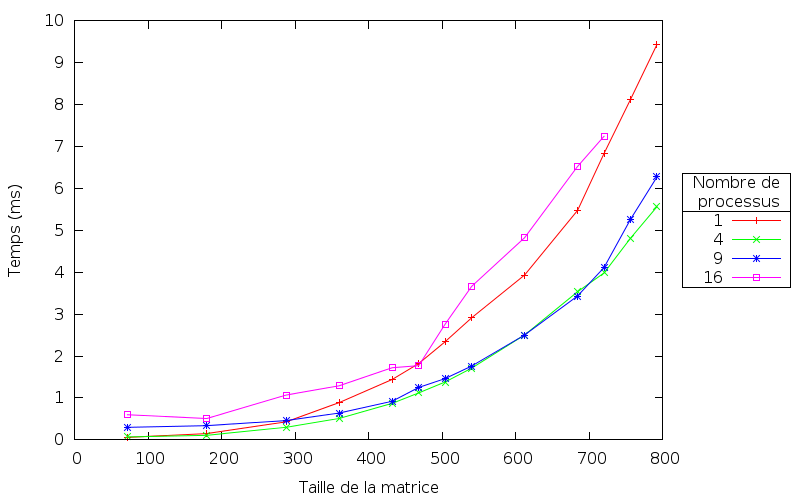
\includegraphics[width=\textwidth]{plot.png}
  \caption{Performance du programme}
  \label{perf}
\end{figure}

En raison de problème sur PLAFRIM, il n'a pas été possible de réaliser les tests de performances sur les fourmis ; les tests ont tout de même été réalisé dessus, la machine étant multicœur. On peut observer les résultats sur la figure \ref{perf}. De manière prévisible, la version n'utilisant qu'un processus devient rapidement lente au fur et à mesure que la dimension de l'entrée augmente. La plateforme semble optimisée pour 4 processus, même si l'exécution avec 9 processus reste proche au début. Avec 16 processus, on constate une dégradation des performances, sûrement liée au surcoût de la création et de l'ordonnancement des processus qui ne peut pas être compensé par une meilleure exécution parallèle, car un nombre limité de processus peuvent être exécuté en même temps, nombre inférieur à 16.
\section{Conclusion}

MPI a permis de réaliser de manière relativement simple un algorithme distribué en s'occupant lui même de tout ce qui a trait à ce caractère distribué, de la création des processus à la leur terminaison en passant par les communications entre eux. Ainsi, un problème ayant une complexité importante, la multiplication matricielle, a pu se résoudre avec des temps de calculs plus modestes, comme les test de performances ont pu le montrer. En outre, en ayant une bonne vision des étapes de calculs et des mécanismes offerts par la bibliothèque il n'était pas plus difficile qu'en séquentiel d'implémenter l'algorithme ; même si bien évidemment il a fallu acquérir cette vision des étapes de calculs et des mécanismes fournis par MPI, chose dans les faits non triviale sans pour autant être d'une difficulté rédhibitoire. Les deux principaux points auxquels il a fallu prendre garde furent la gestion des communications afin que chacun reçoive ce qu'il est sensé recevoir, et la définition du travail effectué par le processus, découlant en droite ligne de l'algorithme.

\end{document}
